\section{Equilibrium properties}

First, we study the equilibrium properties by means of Monte-Carlo simulations.

We start our simulations by selecting a particle at random, and attempting independently a sequence of a translational and a rotational move. We do it sequentially for all particles along the positive direction of the $z$ axis. In the translational move a particle is displaced along the z-axis by a distance $\delta z$, where $\delta z$ is a random value drawn from a uniform distribution in the range $[-\delta z_{max}, +\delta z_{max}]$, with $\delta z_{max} = 0.5 (\Delta z_\mathrm{min} - \Delta z_0)$. $\Delta z_\mathrm{min}$ is the interparticle distance for which the interaction energy between two aligned dipoles is minimal and $\Delta z_0$ is the interparticle distance for which the potential energy vanishes if we decrease distance starting from $\Delta z_\mathrm{min}$, corresponding to the filled symbols in \figref{fig:interaction_energy}. For the rotational move a new orientation is chosen uniformly at random. Each of these moves is \textcolor{red}{Yes, I calculate the probability for rotation and translation separately} accepted with probability $\mathrm{min} \left\{1, \, \exp(\Delta E / k_BT) \right\}$, $\Delta E$ is the change in potential energy due to the trial move.

For the sake of simplicity, we restrict interactions to the first neighbors and consider periodic boundary conditions.

To generate the initial configuration, dipolar particles were regularly distributed along $z$ axis, with an interparticle distance $d = \frac{D}{\rho}$, and then subjected to a random displacement drawn from a uniform distribution in the range $[-d/4, d/4]$. The orientation of the dipoles was generated uniformly at random.

We define the diameter of the particles $D=\Delta z_\mathrm{min}$, and consider different values for the density, $\rho= ND/L = \left(0.25, 0.50, 0.75\right)$, where $L$ is the length of the simulation box along $z$ axis and $N$ is the number of particles. To evaluate possible finite-size effects, for each density, we considered three different number of particles, $N = \left(1600, 3200, 6400 \right)$, and we adjusted $L$ accordingly.

Each Monte-Carlo simulation was relaxed for $\Delta = 3 \cdot 10^5$ Monte-Carlo sweeps, and afterwards different quantities were measured for every $\Delta$ sweeps, obtaining $10$ uncorrelated samples. 

The dipole-dipole interaction encourages co-alignment of particles dipole moments, and therefore we first look into the dependence on $k_BT$ of the nematic order parameter $S$ defined as
\begin{equation}
\label{eq:nematic_order_parameter}
	S = \frac{3 \langle\cos^2 \theta\rangle - 1}{2}
	,
\end{equation}
where $\theta$ it the angle between particle dipole moment and $z$ axis, while angle brackets denote ensemble averages over all particles.

First thing to note is that with decrease of $k_BT$ the order parameter increases. As we can see in the \figref{fig:op_kbt}, we can distinguish high $(\rho \geq 0.5)$ and low $(\rho = 0.25)$ density regimes. For the high density, the results suggest exponential dependence of order parameter on $k_BT$, however on close examination we see small deviations at the high $k_BT$. \figref{fig:op_kbt} shows that curvature of temperature dependence of $\log(S)$ decreases with increase in density. That allows us to expect purely exponential temperature dependence of the order parameter for $\rho > 0.75$. If we try to analyze temperature dependence of order parameter in the form of $S(k_BT) \propto \exp\left[-T/T^* \right]$, we can find $T^* = 1.25$. \textcolor{red}{I calculated the slope of the $\ln(S)$ for $\rho = 0.75$. Also, if I calculate the slope of $\ln(S)$ for lower $\rho$, in the area of $k_BT \leq 1.5$, I get $T^* = (0.3, 0.5)$ for $\rho = (0.25, 0.5)$ respectively. Not sure if if worth including - I don't have data for such a low $k_BT$}

Comparing the results obtained with different system sizes, we do not observe any systematic dependences, and the fluctuations around average values are of order of $10^{-4}$ for any given $k_BT$. On this basis we conclude that we find do not find significant finite-size effects.

\begin{figure}[t]
\centering
	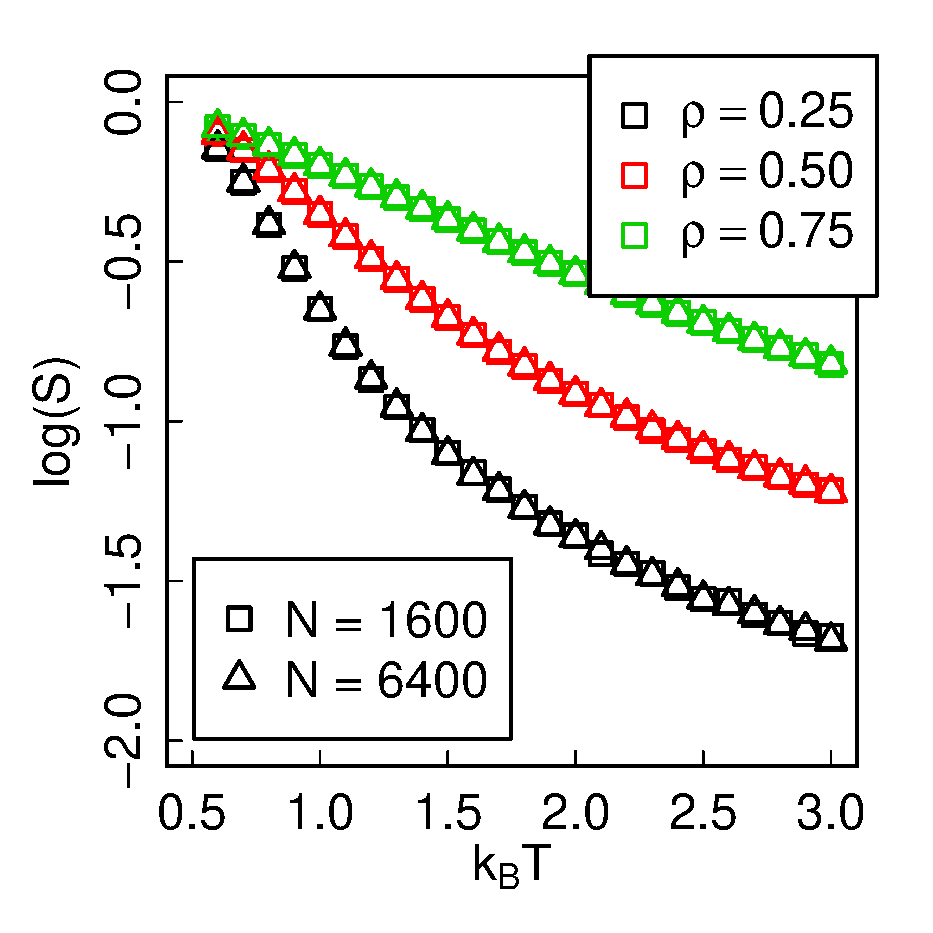
\includegraphics[width=0.7\columnwidth]{Images/op_eq_log}
	\caption{Temperature dependence of the order parameter defined by Eq.~\eqref{eq:nematic_order_parameter}. Triangles are results for $N = 6400$ and squares are for $N = 1600$ particles. We observe no significant dependence on the system size. The points are obtained by means of Monte-Carlo simulations, and are averages over $400$ samples.}
	\label{fig:op_kbt}
\end{figure}

The increase of order parameter signifies increase in co-alignment of particles with each other and in our case with $z$ axis. In case of asymmetric particles we cant automatically connect increase of order parameter to emergence of long-range order in the system. Since interparticle interaction is symmetrical in our case, to further investigate the internal structure of the system, we analyzed the orientation correlation of particles as function of distance between them:
\begin{equation}
\label{eq:distance_correlation}
	C(\Delta z) = \langle\cos \theta_i \cos \theta_j\rangle
	,
\end{equation}
where $\theta_i$ and $\theta_j$ are the angles between spatial axis and dipole moments of particles for which $\Delta z - \delta < |z_j - z_i| \leq \Delta z + \delta$, where $2\delta$ is a predefined space sampling. Angle brackets denotes ensemble-averaging over all particles in all samples which satisfy distance criteria.

For all observed range of simulation parameters the correlation decays exponentially with the distance, as shown in \figref{fig:dist_corr_eq}. The dots are obtained with $\delta = 0.25D$, and are averaged over $400$ samples with $N = 6400$ particles. Lines are obtained by linear fit in the range $0.01 < C(\Delta z) < 0.45$ \textcolor{red}{The range is for $C(\Delta z)$, and the rationality is that for any $k_BT$ and $\rho$ the dependence looks linear and doesn't have strong fluctuations}.
\begin{figure*}[t]
\centering
\begin{minipage}[c]{0.32\textwidth}
	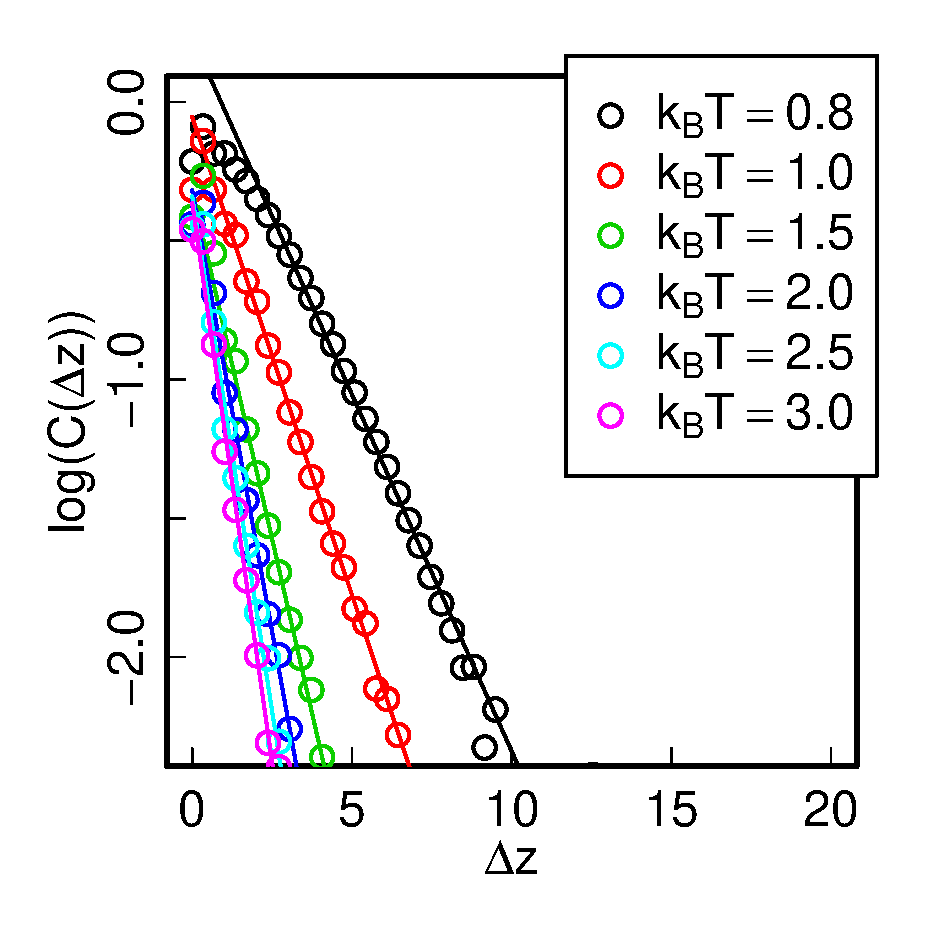
\includegraphics[width=\textwidth]{Images/distCor_25}
\end{minipage}
\begin{minipage}[c]{0.32\textwidth}
	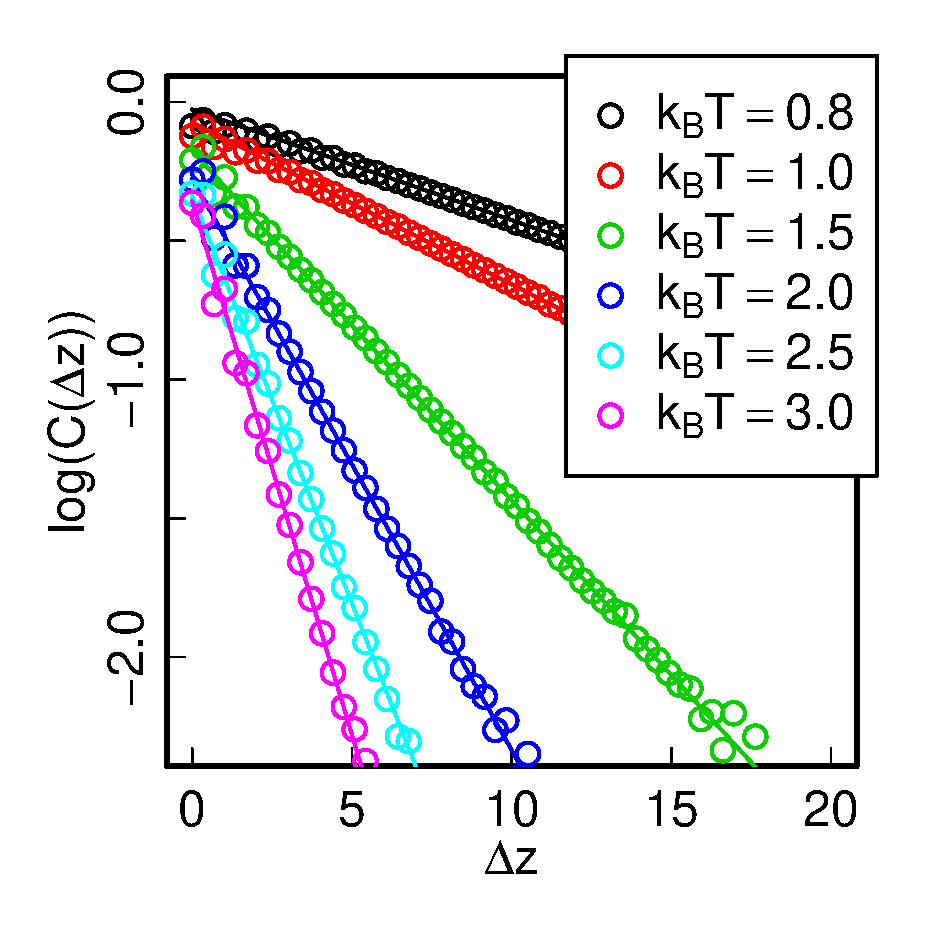
\includegraphics[width=\textwidth]{Images/distCor_75}
\end{minipage}
\begin{minipage}[c]{0.32\textwidth}
	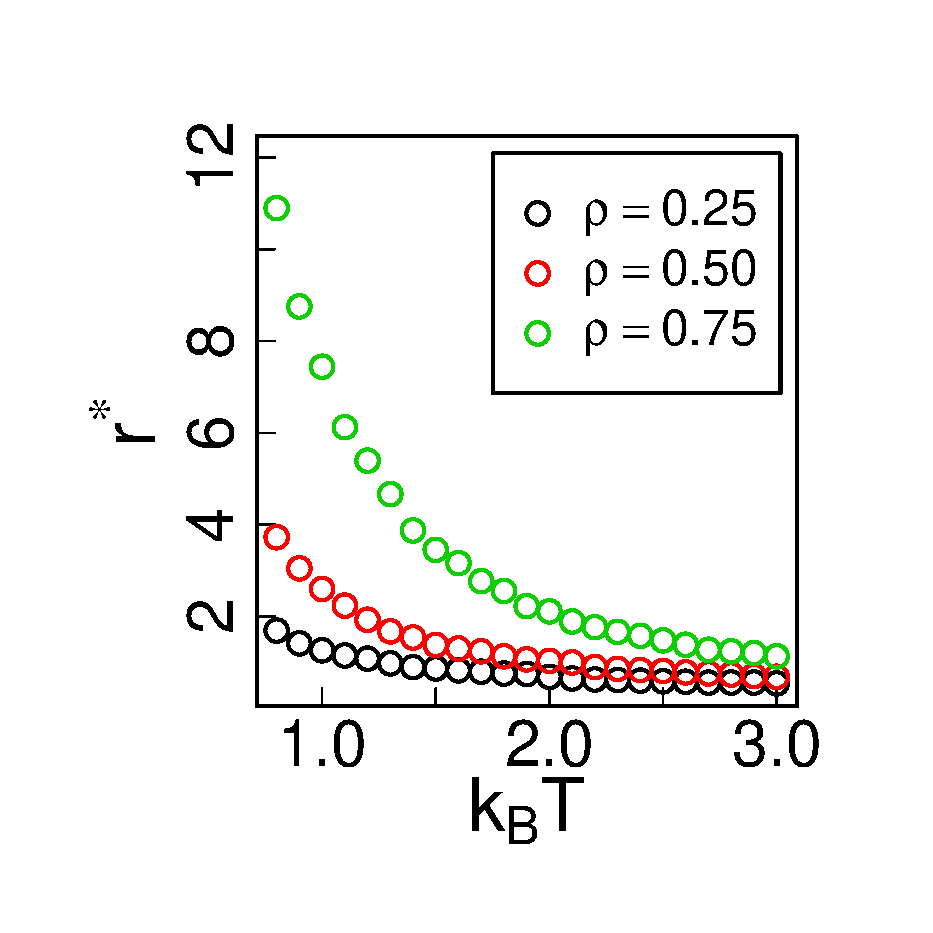
\includegraphics[width=\textwidth]{Images/correlation_length_eq}
\end{minipage}
	\caption{Orientation correlation as function of distance defined by Eq.~\eqref{eq:distance_correlation} at equilibrium for $\rho = 0.25$ (left) and $\rho = 0.75$ (center). The points are calculated for simulations with $N = 6400$ particles and the results are averaged over $400$ samples. Lines are the best (least squares) linear fit to the results in range $0.01 < C(\Delta z) < 0.45$. (right) shows $r^*$ defined by Eq.~\eqref{eq:slopes_def}.}
	\label{fig:dist_corr_eq}
\end{figure*}

The exponential decay of correlation with length for every combination of simulation parameters shows that we do not have emergence of a long range order occurring in the system under study, despite non-zero order parameter observed above. We could now write $C(\Delta z)$ as
\begin{equation}
	\label{eq:slopes_def}
	C(\Delta z) \propto \exp\left[-\Delta z / r^* \right]
\end{equation}
where $r^*$ is the correlation length. The dependence of $r^*$ on the $k_BT$ for different system densities is shown in \figref{fig:dist_corr_eq}, right. We can note the similarity in behavior of order parameter and the correlation length, however, the obtained results suggest power-law increase in correlation length with decrease in $k_BT$ for any given density, as opposed to exponential increase for the order parameter for high density.

